\section{Control Unit (Unité de Contrôle)}

The control unit consists of a 32-bit register and a combinatorial decoder.

\subsection{32-bit Register with Load Instruction (Registre 32-bit avec Commande de Chargement)}

This register will be used to store the state of the processor 
(Processor State Register, PSR).
In this project, we only consider the state which will be 
limited to the value of the \texttt{N flag} of the \textbf{ALU}.
A symbolic representation of this 32-bit register
is shown in Figure \ref{fig:32Register}.

\begin{figure}[htp]
    \centering
    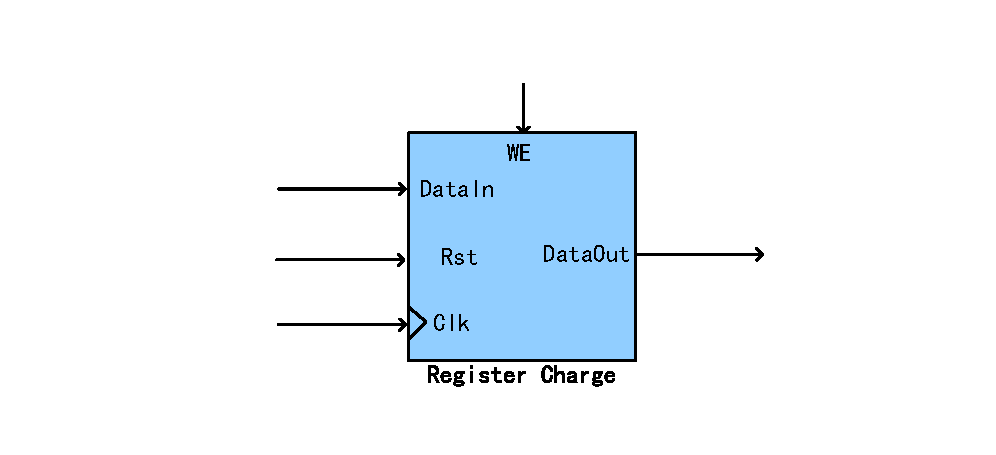
\includegraphics[width=0.4\textwidth]{picture/32Register.pdf}
    \caption{32-bit Register Block Diagram}     
    \label{fig:32Register}
\end{figure}

Where \texttt{DataIn} and \texttt{DataOut} are the 32-bit buses for 
instruction input and outpout respectively, \texttt{WE} is enable signal
for charge command.

Based on the analysis above, we can draw the equation:
\begin{equation*}
    \texttt{DataOut} = \begin{cases}
        \texttt{DataOut} & \texttt{WE} = 0 \\
        \texttt{DataIn} & \texttt{WE} = 1
    \end{cases}
\end{equation*} 

It's not hard to synthesize the code. We show the part of the code of this component in \textbf{Registre\_Charge.vhd}.

\begin{lstlisting}[style=vhdl]
architecture behave of Register_Charge is
begin
    
    process(clk, rst) 
    begin 
        if rst ='1' then 
            DataOut <= (others => '0'); 
        elsif rising_edge(clk) then 
            if WE = '1' then 
                DataOut <= DataIn;	
            end if; 
        end if; 
    end process; 
    
end architecture;
\end{lstlisting}


\subsection{Instruction Decoder (Decodeur d’Instructions)}
\label{sec:Instruction Decoder}

This combinatorial module generates the control signals for 
the processing unit, the instruction management unit, 
as well as the PSR register(32-bit register), which all described
previously.

A symbolic representation of decoder
is shown in Figure \ref{fig:decoder}.

\begin{figure}[htp]
    \centering
    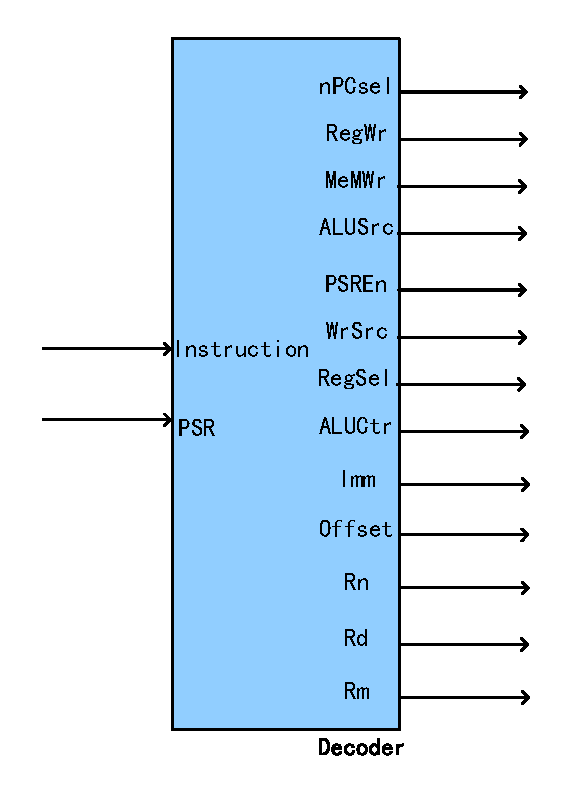
\includegraphics[width=0.4\textwidth]{picture/decoder.pdf}
    \caption{Decoder Block Diagram}     
    \label{fig:decoder}
\end{figure}

The values of these commands depend on the statement retrieved from 
the instruction memory, and possibly the state of the PSR register. 
The structure binary of the different instructions is described 
in the Appendix, and we completed it as Table \ref{tab:command}.

\begin{table}[htp]
    \caption{Commands}
    \label{tab:command}
    \resizebox{\textwidth}{!}
    {
        \begin{tabular}{@{}ccccccccc@{}}
        \toprule
        \textbf{INSTRUCTION} & \textbf{nPCSel} & \textbf{RegWr} & \textbf{ALUSrc} & \textbf{ALUCtr} & \textbf{PSREn} & \textbf{MemWr} & \textbf{WrSrc} & \textbf{RegSel} \\ \midrule
        ADDi                 &       0         &          1     &      1          &       00         &     0          &       0        &      0         &   0             \\
        ADDr                 &       0         &         1      &      0          &      00          &      0         &        0       &       0        &  0              \\
        BAL                  &         1       &        0       &     0           &    00            &     0          &     0          &     0          &    0            \\
        BLT                  &         0       &           0    &          0      &      00         &       0        &         0      &        0       &      0          \\
        CMP                  &       0         &    0           &    1            &    10           &     1          &     0          &        0       &   0             \\
        LDR                  &         0       &      1         &         1       &      00          &        0       &         0      &       1        &    0            \\
        MOV                  &         0       &       1        &           1     &         10       &       0        &     0          &        0       &      0          \\
        STR                  &         0       &   0            &       1         &       00         &       0        &       1        &       0        &      1          \\ \bottomrule
        \end{tabular}
    }
\end{table}

The ARM instruction set formats are shown in the Appendices \ref{AppendicesA}.

And we focus on the instructions such as
\begin{lstlisting}[style = Arm, columns = fixed]
    LDR Rd, [Rn, #Offset]   @ LDR (Immediate)
    STR Rd, [Rn, #Offset]   @ STD (Immediate)
    B       label           @ B (Always)
    BLT     label           @ B (If Less Than)
\end{lstlisting}

These instruction set formats are shown as Figure \ref{fig:AISFIP}, and more detailed information will be shown in the Appendices \ref{AppendicesA}.

\begin{figure}[htp]
    \centering
    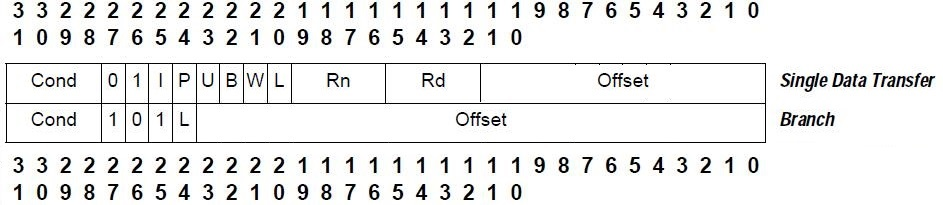
\includegraphics[width=1\textwidth]{picture/ARM instruction set formats in project.jpg}
    \caption{Load, Store and Branch Instruction Set Formats}     
    \label{fig:AISFIP}
\end{figure}

The single data transfer instructions are used to load or store single bytes or words of
data. The memory address used in the transfer is calculated by adding an offset to or
subtracting an offset from a base register.

The result of this calculation may be written back into the base register if auto-indexing
is required.

Branch instructions contain a signed 2’s complement 24 bit offset. This is shifted left
two bits, sign extended to 32 bits, and added to the PC. The instruction can therefore
specify a branch of +/- 32Mbytes. The branch offset must take account of the prefetch
operation, which causes the PC to be 2 words (8 bytes) ahead of the current instruction.
Branches beyond +/- 32Mbytes must use an offset or absolute destination which has
been previously loaded into a register. In this case the PC should be manually saved in
R14 if a Branch with Link type operation is required.

Thus, for these 4 instructions, bit assignments are as follow:\\
\begin{table}[h!]
    \centering
    \caption{LDR (Immediate) Bit Assignment}
    \label{tab:LDRBA}
    \begin{tabular}{|cccc|cccccccc|ccc|ccc|ccc|}
    \hline
    31 & 30 & 29 & 28 & 27 & 26                     & 25                     & 24                     & 23                     & 22                     & 21                     & 20 & 19     & ...    & 16    & 15     & ...    & 12    & 11      & ...      & 0      \\ \hline
    1  & 1  & 1  & 0  & 0  & \multicolumn{1}{c|}{1} & \multicolumn{1}{c|}{1} & \multicolumn{1}{c|}{0} & \multicolumn{1}{c|}{0} & \multicolumn{1}{c|}{0} & \multicolumn{1}{c|}{0} & 1  & \multicolumn{3}{c|}{Rn} & \multicolumn{3}{c|}{Rd} & \multicolumn{3}{c|}{Offset} \\ \hline
    \end{tabular}
\end{table}

\begin{table}[h!]
    \centering
    \caption{STR (Immediate) Bit Assignment}
    \label{tab:STRBA}
    \begin{tabular}{|cccc|cccccccc|ccc|ccc|ccc|}
    \hline
    31 & 30 & 29 & 28 & 27 & 26                     & 25                     & 24                     & 23                     & 22                     & 21                     & 20 & 19     & ...    & 16    & 15     & ...    & 12    & 11      & ...      & 0      \\ \hline
    1  & 1  & 1  & 0  & 0  & \multicolumn{1}{c|}{1} & \multicolumn{1}{c|}{1} & \multicolumn{1}{c|}{0} & \multicolumn{1}{c|}{0} & \multicolumn{1}{c|}{0} & \multicolumn{1}{c|}{0} & 0  & \multicolumn{3}{c|}{Rn} & \multicolumn{3}{c|}{Rd} & \multicolumn{3}{c|}{Offset} \\ \hline
    \end{tabular}
\end{table}

\begin{table}[h!]
    \centering
    \caption{B (Always) Bit Assignment}
    \label{tab:BALBA}
    \begin{tabular}{|cccc|cccc|ccllllllllllc|}
    \hline
    31 & 30 & 29 & 28 & 27 & 26 & 25                     & 24 & 23 & ...    &  ...   &   ...  & ... & ... & ... & ... & ... & ... & ... & ... & 0 \\ \hline
    1  & 1  & 1  & 0  & 1  & 0  & \multicolumn{1}{c|}{1} & 0  & \multicolumn{13}{c|}{Offset}                                             \\ \hline
    \end{tabular}
    
\end{table}

\begin{table}[h!]
    \centering
    \caption{B (If Less Than) Bit Assignment}
    \label{tab:BLTBA}
    \begin{tabular}{|cccc|cccc|ccllllllllllc|}
    \hline
    31 & 30 & 29 & 28 & 27 & 26 & 25                     & 24 & 23 & ...    &  ...   &   ...  & ... & ... & ... & ... & ... & ... & ... & ... & 0 \\ \hline
    1  & 0  & 1  & 1  & 1  & 0  & \multicolumn{1}{c|}{1} & 0  & \multicolumn{13}{c|}{Offset}                                             \\ \hline
    \end{tabular}
\end{table}

\vspace{3cm}
Based on the analysis above, we build the code of \textbf{Decoder.vhd}.
\begin{lstlisting}[style=vhdl,columns=fixed, breaklines]
entity Decoder  is
	port(
		Instruction, PSRout : in std_logic_vector(31 downto 0);
		Offset : out std_logic_vector(23 downto 0);
		Immediate : out std_logic_vector(7 downto 0);
		Rn, Rm, Rd : out std_logic_vector(3 downto 0);
		ALUctr : out std_logic_vector(1 downto 0);
		nPCsel, RegWr, ALUsrc, PSRen, MemWr, WrSrc, RegSel : out std_logic
	);
end entity;

architecture behave of Decoder  is
	type enum_instruction is (MOV, ADDi, ADDr, CMP, LDR, STR, BAL, BLT, XXX);
	signal instr_courante: enum_instruction;
begin

	Immediate <= Instruction(7  downto  0);
	Offset    <= Instruction(23 downto  0);
	Rn        <= Instruction(19 downto 16);
	Rd        <= Instruction(15 downto 12);
	Rm        <= Instruction(3  downto  0);
	process(Instruction)
	begin
		case Instruction(27 downto 26) is
			when "00"   => 
				case Instruction(25 downto 23) is
					when "001"          => instr_courante <= ADDr;
					when "101"          => 
						case Instruction(29) is
							when '1'    => instr_courante <= ADDi;
							when others => instr_courante <= XXX;
						end case;
					when "110" | "010"  => instr_courante <= CMP;
					when "111"          => instr_courante <= MOV;
					when others         => instr_courante <= XXX;
				end case;
									
			when "01"   => 
				case Instruction(20) is
					when '0'    => 
						case Instruction(29) is
							when '1'    => instr_courante <= STR;
							when others => instr_courante <= XXX;
						end case;
					when '1'    => instr_courante <= LDR;
					when others => instr_courante <= XXX;
				end case;
									
			when "10"   => 
				case Instruction(29 downto 28) is
					when "10"    => instr_courante <= BAL;
					when "11"    => instr_courante <= BLT;
					when others  => instr_courante <= XXX;
				end case;					   
			when others => instr_courante <= XXX;
		end case; 
	end process;
		
	process(instr_courante)
	begin
		-- MemWr et RegSel
		case instr_courante is
			when STR 	=> 	MemWr  <= '1';
						   	ALUSrc <= '1'; 
						   	RegSel <= '1';
			when others => 	MemWr  <= '0';
							RegSel <= '0';			
		end case;
		
		-- WrSrc
		case instr_courante is
			when LDR	=> 	WrSrc <= '1';
			when others => 	WrSrc <= '0';
		end case;
		
		-- PSRen et UALctr
		case instr_courante is
			when CMP 	=> 	PSRen  <= '1';
							ALUctr <= "10";
			when MOV	=> 	PSRen  <= '0';
							ALUctr <= "01";
			when others => 	PSRen  <= '0';
							ALUctr <= "00";
		end case;
		
		--UALsrc
		case instr_courante is
			when ADDr   => 	ALUsrc <= '0';
			when CMP    => 	ALUsrc <= Instruction(25);
			when others => 	ALUsrc <= '1';
		end case;
		
		-- RegWr
		case instr_courante is
			when ADDi | ADDr | LDR | MOV => RegWr <= '1';
			when others                  => RegWr <= '0';
		end case;
		
		-- nPCsel
		case instr_courante is
			when BAL    => nPCsel <= '1';
			when BLT    => nPCsel <= PSRout(31);
			when others => nPCsel <= '0';
		end case;
		
	end process;

end architecture;
\end{lstlisting}


At this point, all the components have been constructed. 
In the next part, we will try to assemble the processor by using these components.
